\documentclass[a4paper,10pt]{article}%
\input{commands.tex}%

\author{Peter Bonventre, Lu\'is A. Pereira}%
\title{Genuine equivariant operads}%

\usepackage{showkeys}%

\usepackage{stmaryrd}

\usepackage{geometry}

\usepackage{tikz}%
\tikzset{%
  treenode/.style = {shape=rectangle, rounded corners,%
                     draw, align=center,%
                     top color=white, bottom color=blue!20},%
  root/.style     = {treenode, font=\Large, bottom color=red!30},%
  env/.style      = {treenode, font=\ttfamily\normalsize},%
  dummy/.style    = {circle,draw,inner sep=0pt,minimum size=2mm}%
}%

\usetikzlibrary[decorations.pathreplacing]

\begin{document}	\maketitle%


\abstract{We build new algebraic structures, which we call genuine equivariant operads, which can be thought of as a hybrid between equivariant operads and coefficient systems.
We then prove an Elmendorf type theorem stating that equivariant operads, with their graph model structure, are equivalent to genuine equivariant operads with their projective model structure.

As an application, we build explicit models for the $N_{\infty}$-operads of Blumberg and Hill.
}

\tableofcontents

\section{Introduction}

No content yet.



\section{Planar and tall maps}

\subsection{Planar structures}


Throughout we will work with trees possessing \textit{planar structures} or, more intuitively, trees embedded into the plane.

Our preferred model for trees will be that of broad posets first introduced by Weiss in \cite{We12} and further worked out by the second author in \cite{Pe16b}. We now define planar structures in this context.


\begin{definition}\label{PLANARIZE DEF}
	Let $T \in \Omega$ be a tree. A \textit{planar structure} of $T$ is an extension of the descendancy partial order $\leq_d$ to a total order $\leq_p$ such that: 
	\begin{itemize}
		\item \textit{Planar}: if $e \leq_p f$ and $e \nleq_d f$ then 
		$g \leq_d f$ implies $e \leq_p g$.
	\end{itemize} 
\end{definition}


\begin{example}
An example of a planar structure on a tree $T$ follows, with $\leq_r$ encoded by the number labels.
\begin{equation}\label{PLANAREX EQ}
	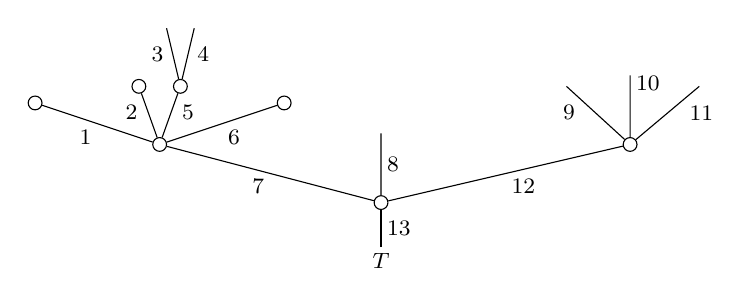
\begin{tikzpicture}[grow=up,auto,level distance=2.1em,
	every node/.style = {font=\footnotesize,inner sep=2pt},
	dummy/.style={circle,draw,inner sep=0pt,minimum size=1.75mm}]
		\node at (0,0) {$T$}
			child{node [dummy] {}
				child[sibling distance = 9em]{node [dummy] {}
					child[sibling distance = 2.5em]{
					edge from parent node [near end,swap] {$11$}}
					child[level distance=2.5em]{
					edge from parent node [very near end,swap] {$10$}}				
					child[sibling distance = 2.3em]{
					edge from parent node [near end] {$9$}}
				edge from parent node [swap] {12}}
				child[level distance =2.5em]{
				edge from parent node [swap] {$8$}}
				child[sibling distance = 8em]{node [dummy] {}
					child[sibling distance =3em, level distance = 1.5 em]{node [dummy] {}
					edge from parent node [swap] {$6$}}
					child[sibling distance = 1.5em]{node [dummy] {}
						child[sibling distance =1em]{
						edge from parent node [swap,near end] {$4$}}
						child[sibling distance =1em]{
						edge from parent node [near end] {$3$}}
					edge from parent node [very near end,swap] {$5$}}
					child[sibling distance =1.5em]{node [dummy] {}
					edge from parent node [very near end] {$2$}}
					child[sibling distance =3em,level distance =1.5em]{node [dummy] {}
					edge from parent node {$1$}}
				edge from parent node {$7$}}
			edge from parent node [swap] {$13$}};
	\end{tikzpicture}
\end{equation}
Intuitively, given a planar depiction of a tree $T$, $e \leq_d f$ holds when the downward path from $e$ passes through $f$
and $e \leq_p f$ holds if either
$e \leq_d f$ or if the downward path from $e$ is to the left of the downward path from $f$ (as measured at the node where the paths intersect).
\end{example}



Intuitively, a planar depiction of a tree amounts to choosing a total order for each of the sets of \textit{input edges} of each node (i.e. those edges immediately above that node).

While we will not need to make this last statement precise, we will nonetheless find it convenient to show that Definition \ref{PLANARIZE DEF} is equivalent to such choosing total orders for each of the sets of input edges.
To do so, we first introduce some notation.


\begin{notation}\label{INPUTPATH NOT}
	Let $T \in \Omega$ be a tree and $e \in T$ and edge. We will denote
	\[ I(e) =\{f \in T \colon e \leq_d f \} \]
and refer to this poset as the \textit{input path of $e$}.
\end{notation}

We will repeatedly use the following, which is a consequence of \cite[Cor. 5.26]{Pe16b}.

\begin{lemma}\label{INCOMPNOTOP}
If $e \leq_d f$, $e \leq_d f'$, then $f,f'$ are $\leq_d$-comparable. 
\end{lemma} 

\begin{proposition}\label{INPUTPATHS PROP}
	Let $T \in \Omega$ be a tree. Then
	\begin{itemize}
		\item[(a)] for any $e \in T$ the finite poset $I(e)$ is totally ordered;
		\item[(b)] the poset $(T,\leq_d)$ has all joins, denoted $\vee$. In fact, $\bigvee_{i} e_i = \min (\bigcap_{i} I(e_i))$.
	\end{itemize}
\end{proposition}

\begin{proof}
	(a) is immediate from Lemma \ref{INCOMPNOTOP}.
To prove (b) we note that 
	$\min (\bigcap_{i} I(e_i))$ exists by (a), and that this is clearly the join $\bigvee{e_i}$.
\end{proof}


\begin{notation}
	Let $T \in \Omega$ be a tree and suppose that $e <_d b$. We will denote by $b^{\uparrow}_e \in T$ the predecessor of $b$ in $I(e)$.
\end{notation}


\begin{proposition}\label{INPUTPREDECESSORPROP PROP}
Suppose $e,f$ are $\leq_d$-incomparable edges of $T$ and write $b= e \vee f$. Then
\begin{itemize}
\item [(a)] $e <_d b$, $f<_d b$ and $b^{\uparrow}_e \neq b^{\uparrow}_f$;
\item [(b)] $b^{\uparrow}_e, b^{\uparrow}_f \in b^{\uparrow}$. In fact $\{b^{\uparrow}_e\} = I(e) \cap b^{\uparrow}$,
$\{b^{\uparrow}_f\} = I(f) \cap b^{\uparrow}$;
\item[(c)] if $e' \leq_d e$, $f' \leq_d f$ then 
$b = e' \vee f'$ and $b^{\uparrow}_{e'} = b^{\uparrow}_{e}$, $b^{\uparrow}_{f'} = b^{\uparrow}_{f}$.
\end{itemize}
\end{proposition}


\begin{proof}
(a) is immediate: the condition $e = g$ (resp. $f = g$) would imply $f \leq_d e$ (resp. $e \leq_d f$)
while the condition $b^{\uparrow}_e = b^{\uparrow}_f$ would provide a predecessor of $b$ in $I(e) \cap I(f)$. 

For (b), note that any relation $a <_d b$ factors as 
$a \leq_d b^{\star}_a <_d b$ for some unique $b^{\**}_a \in b^{\uparrow}$, where uniqueness follows from Lemma \ref{INCOMPNOTOP}. Choosing $a=e$ implies $I(e) \cap b^{\uparrow} = \{b^{\**}_e\}$ and letting $a$ range over edges such that $e \leq_d a <_d b$ shows that $b^{\**}_e$ is in fact the predecessor of $b$.

To prove (c) one reduces to the case $e'=e$, in which case it suffices to check $I(e) \cap I(f') = I(e) \cap I(f)$. But if it were otherwise there would exist an edge $a$ satisfying
$f' \leq_d a <_d f$ and $e \leq_d a$, and this would imply $e \leq_d f$, contradicting our hypothesis.
\end{proof}



\begin{proposition}
\label{TERNARYJOIN PROP}
Let $c = e_1 \vee e_2 \vee e_3$.
Then $c = e_i \vee e_j$ iff $c^{\uparrow}_{e_i} \neq c^{\uparrow}_{e_j}$.

Therefore, all ternary joins in $(T,\leq_d)$ are binary, i.e.
\begin{equation}\label{TERNJOIN EQ}
	c = e_1 \vee e_2 \vee e_3 = e_i \vee e_j
\end{equation}
for some $1\leq i <j \leq 3$, and
(\ref{TERNJOIN EQ}) fails for 
 at most one choice of $1\leq i <j \leq 3$.
\end{proposition}


\begin{proof}
If $c^{\uparrow}_{e_i} \neq c^{\uparrow}_{e_j}$ then
$c = \min\left(I(e_i) \cap I(e_j)\right) = e_i \vee e_j$, whereas the converse follows from Proposition \ref{INPUTPREDECESSORPROP PROP}(a).

The ``therefore'' part follows by noting that 
$c^{\uparrow}_{e_1}$, $c^{\uparrow}_{e_2}$, $c^{\uparrow}_{e_3}$
can not all coincide, or else $c$ would not be the minimum of
$I(e_1) \cap I(e_2) \cap I(e_3)$. 
\end{proof}


\begin{example} In the following example $b = e \vee f$, $c = e \vee f \vee g$, $c^{\uparrow}_e= c^{\uparrow}_f =b$.
\[
	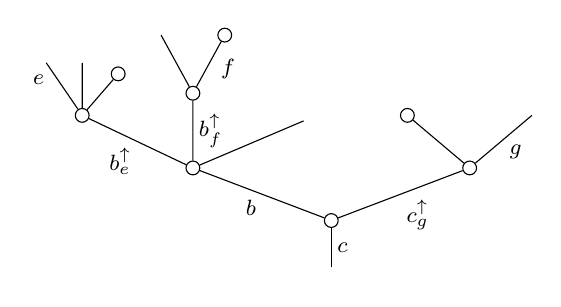
\begin{tikzpicture}[grow=up,auto,level distance=1.9em,
	every node/.style = {font=\footnotesize,inner sep=2pt},
	dummy/.style={circle,draw,inner sep=0pt,minimum size=1.75mm}]
		\node at (0,0) {}
			child{node [dummy] {}
				child[sibling distance = 10em]{node [dummy] {}
					child[sibling distance = 4.5em]{
					edge from parent node [swap] {$g$}}
					child[sibling distance = 4.5em]{node [dummy] {}}
				edge from parent node [swap] {$c_g^{\uparrow}$}}
				child[sibling distance = 10em]{node [dummy] {}
					child[sibling distance = 4em,level distance=1.7em]
					child[sibling distance = 1.5em,level distance=2.7em]{node [dummy] {}
						child[level distance=2.1em,sibling distance = 2.3em]{node [dummy] {}
						edge from parent node [near end,swap] {$f$}}		
						child[level distance=2.1em,sibling distance = 2.3em]{
						edge from parent node [near end] {}}
					edge from parent node [swap] {$b^{\uparrow}_{f}$}}
					child[sibling distance = 4em]{node [dummy] {}
						child[sibling distance =1.3em, level distance = 1.5 em]{node [dummy]  {}
						edge from parent node [swap] {}}
						child[sibling distance = 1.3em]{
						edge from parent node [very near end,swap] {}}
						child[sibling distance =1.3em]{
						edge from parent node [very near end] {$e$}}
					edge from parent node {$b^{\uparrow}_e$}}
				edge from parent node {$b$}}
			edge from parent node [swap] {$c$}};
	\end{tikzpicture}
\]
\end{example}

\begin{notation}
	Given a set $S$ of size $n$ we write
	$\textsf{Ord}(S) \simeq \mathsf{Iso}(S,\{1,\cdots,n\})$. We will usually abuse notation by regarding its objects as pairs $(S,\leq)$ where $\leq$ is a total order in $S$.
\end{notation}


\begin{proposition}\label{PLANARIZATIONCHAR PROP}
	Let $T \in \Omega$ be a tree. There is a bijection
	\begin{equation}\label{PLANAR EQ}
	\begin{tikzcd}[row sep = 0.5em]
		\{\text{planar structures }(T,\leq_p)\} \ar[r] &
		\prod_{(a^{\uparrow} \leq a) \in V(T)} \mathsf{Ord}(a^{\uparrow}) \\
		\leq_p \ar[mapsto]{r} & (\leq_p|_{a^{\uparrow}})
	\end{tikzcd}	
	\end{equation}
\end{proposition}


\begin{proof}
We will keep the setup of Proposition \ref{INPUTPREDECESSORPROP PROP} throughout: $e, f$ are $\leq_d$-incomparable edges and we write $b = e \vee f$. 

	We first show that (\ref{PLANAR EQ}) is injective, i.e. that the restrictions $\leq_p|_{a^{\uparrow}}$ determine if 
	$e <_p f$ holds or not.
If $b^{\uparrow}_e <_p b^{\uparrow}_f$, the relations
$e \leq_d b^{\uparrow}_e <_p b^{\uparrow}_f \geq_d f$
and Definition \ref{PLANARIZE DEF} imply it must be $e <_p f$.
Dually, if $b^{\uparrow}_f <_p b^{\uparrow}_e$ then 
$f <_p e$. Thus 
$b^{\uparrow}_e <_p b^{\uparrow}_f \Leftrightarrow e <_p f$ and hence (\ref{PLANAR EQ}) is indeed injective.

To check that (\ref{PLANAR EQ}) is surjective, it suffices (recall that $e,f$ are assumed $\leq_d$-incomparable) to check that
defining $e \leq_p f$ to hold iff $b^{\uparrow}_e < b^{\uparrow}_f$ holds in $b^{\uparrow}$ yields a planar structure.

Antisymmetry and the total order conditions are immediate, and it thus remains to check the transitivity and planar conditions.
Transitivity of $\leq_p$ in the case $e' \leq_d e <_p f$ and the planar condition, which is the case $e <_p f \geq_d f'$, follow from Proposition \ref{INPUTPREDECESSORPROP PROP}(c). Transitivity of $\leq_p$ in the case $e <_p f \leq_d f'$
follows since either $e \leq_d f'$ or else $e,f'$ are $\leq_d$-incomparable, in which case one can apply \ref{INPUTPREDECESSORPROP PROP}(c) with the roles of $f,f'$ reversed.

It remains to check transitivity in the hardest case, that of 
$e <_p f <_p g$ with $\leq_d$-incomparable $f,g$.
We write $c = e \vee f \vee g$.
By the ``therefore'' part of Proposition \ref{TERNARYJOIN PROP}, either
\begin{inparaenum}
	\item[(i)] $e \vee f <_d c$, in which case 
	Proposition \ref{TERNARYJOIN PROP}
	implies 
	$c^{\uparrow}_e = c^{\uparrow}_f$ and transitivity follows;
	\item[(ii)] $f \vee g <_d c$, which follows just as (i);
	\item[(iii)]  
$e \vee f = f \vee g =c$, in which case 
$c^{\uparrow}_e <
c^{\uparrow}_f <
c^{\uparrow}_g $ in $c^{\uparrow}$
so that $c^{\uparrow}_e \neq c^{\uparrow}_g$ and by Proposition \ref{TERNARYJOIN PROP} it is also 
$e \vee g = c$ and transitivity follows.
\end{inparaenum}
\end{proof}


\begin{remark}\label{FORESTPLAN REM}
	Definition \ref{PLANARIZE DEF} readily extends to forests $F \in \Phi$. The analogue of Proposition \ref{PLANARIZATIONCHAR PROP} then states that the data of a planar structure is 
equivalent to total orderings of the nodes of $F$ together with a total ordering of its set of roots.
Indeed, this follows by either adapting the proof above or by noting that planar structures on $F$ are clearly in bijection with planar structures on the join tree $F \star \eta$ 
(cf. \cite[Def. 7.44]{Pe16b}), which adds a single edge $\eta$ to $F$, serving as the (unique) root of $F \star \eta$.
\end{remark}


When discussing the substitution procedure in \S \ref{SUBS SEC} we will find it convenient to work with a model for the category $\Omega$ that possesses exactly one representative of each possible planar structure on each tree or, more precisely, such that the only isomorphisms preserving the planar structures are the identities. On the other hand, using such a model for $\Omega$ throughout would, among other issues, make the discussion of faces in \S \ref{OUTTALL SEC} rather awkward.
We now outline our conventions to address such issues.


Let $\Omega^p$, the category of \textit{planarized trees}, denote the category with objects pairs $T_{\leq_p}=(T,\leq_p)$ of trees together with a planar structure  and morphisms the \textit{underlying} maps of trees (so that the planar structures are ignored).
There is a full subcategory $\Omega^s \hookrightarrow \Omega^p$, whose objects we call \textit{standard models}, of those $T_{\leq_p}$ whose underlying set is one of the sets $\underline{n} = \{1,2,\cdots,n\}$ and for which $\leq_p$ coincides with the canonical order. 
\begin{example}\label{STANDMODEL EX}
	Some examples of standard models, i.e. objects of $\Omega^s$, follow (further, (\ref{PLANAREX EQ}) can also be interpreted as such an example).
\begin{equation}\label{PLANAROMEGAEX1 EQ}
	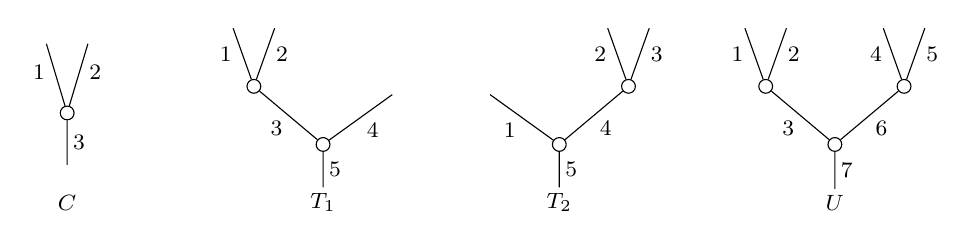
\begin{tikzpicture}[grow=up,auto,level distance=2.1em,
	every node/.style = {font=\footnotesize,inner sep=2pt},
	dummy/.style={circle,draw,inner sep=0pt,minimum size=1.75mm}]
		\node at (-0.25,0) {$C$};
		\node at (-0.25,0.4) {}
			child{node [dummy] {}
				child[sibling distance = 1.5em,level distance= 2.5em]{
				edge from parent node [swap, near end] {$2$}}
				child[sibling distance = 1.5em,level distance= 2.5em]{
				edge from parent node [near end] {$1$}}
			edge from parent node [swap] {$3$}};
		\node at (3,0) {$T_1$}
			child{node [dummy] {}
				child[sibling distance = 5em, level distance=1.8em]{
				edge from parent node [swap] {$4$}}
				child[sibling distance = 5em]{node [dummy] {}
					child[sibling distance = 1.5em]{
					edge from parent node [swap,near end] {$2$}}
					child[sibling distance = 1.5em]{
					edge from parent node [near end] {$1$}}
				edge from parent node {$3$}}
			edge from parent node [swap] {$5$}};
		\node at (6,0) {$T_2$}
			child{node [dummy] {}
				child[sibling distance = 5em]{node [dummy] {}
					child[sibling distance = 1.5em]{
					edge from parent node [swap,near end] {$3$}}
					child[sibling distance = 1.5em]{
					edge from parent node [near end] {$2$}}
				edge from parent node [swap] {$4$}}
				child[sibling distance = 5em, level distance=1.8em]{
				edge from parent node {$1$}}
			edge from parent node [swap] {$5$}};
		\node at  (9.5,0) {$U$}
			child{node [dummy] {}
				child[sibling distance = 5em]{node [dummy] {}
					child[sibling distance = 1.5em]{
					edge from parent node [swap,near end] {$5$}}
					child[sibling distance = 1.5em]{
					edge from parent node [near end] {$4$}}
				edge from parent node [swap] {$6$}}
				child[sibling distance = 5em]{node [dummy] {}
					child[sibling distance = 1.5em]{
					edge from parent node [swap,near end] {$2$}}
					child[sibling distance = 1.5em]{
					edge from parent node [near end] {$1$}}
				edge from parent node {$3$}}
			edge from parent node [swap] {$7$}};
	\end{tikzpicture}
\end{equation}
Here $T_1$ and $T_2$ are isomorphic to each other but not isomorphic to any other standard model in $\Omega^s$ while both $C$ and $U$ are the unique objects in their isomorphism classes. 
\end{example}


Given $T_{\leq_p} \in \Omega^p$ there is an obvious standard model $T_{\leq_p}^s \in \Omega^s$ given by replacing each edge by its order following $\leq_p$. Indeed, this defines a retraction 
$(\minus)^s \colon \Omega^p \to \Omega^s$
and a natural transformation 
$\sigma \colon id \Rightarrow (\minus)^s$
given by isomorphisms preserving the planar structure
(in fact, the pair $\left((\minus)^s, \sigma \right)$ is clearly unique).


\begin{convention}\label{PLANARCONV CON}
	From now on, we will write simply $\Omega$, $\Omega_G$ to denote the categories $\Omega^s$, $\Omega_G^s$ of standard models (where planar structures are defined in the underlying forest as in Remark \ref{FORESTPLAN REM}). 
Similarly $\mathsf{O}_G$ will denote the model $\mathsf{O}_G^s$ for the orbital category whose objects are the orbital $G$-sets whose underlying set is one of the sets $\underline{n} = \{1,2,\cdots,n\}$.

Therefore, whenever one of our constructions produces an object/diagram in $\Omega^p$, $\Omega^p_G$, $\mathsf{O}_G^p$ (of trees, $G$-trees, orbital $G$-sets with a planarization/total order) we will hence implicitly reinterpret it by using the standardization functor $(\minus)^s$.
\end{convention}

\begin{example}
To illustrate our convention, we consider the trees in Example \ref{STANDMODEL EX}. 

One has subfaces
$F_1 \subset F_2 \subset U$
where $F_1$ is the subtree with edge set $\{3,6,7\}$ and 
$F_2$ is the subtree with edge set $\{1,2,3,6,7\}$, both with inherited tree and planar structures. 
Applying $(\minus)^s$ to the inclusion diagram on the left below then yields a diagram as on the right.
\[
\begin{tikzcd}[row sep = 0.5em,column sep =1.3em]
	F_1 \ar[hookrightarrow]{rr} \ar[hookrightarrow]{rd} & & U & &&
	C \ar{rr} \ar{rd} & & U
\\
	& F_2 \ar[hookrightarrow]{ru} & & &&
	& T_1 \ar{ru}
\end{tikzcd}
\]
Similarly, let $\leq_{(12)}$ and $\leq_{(45)}$ denote alternate planar structures for $U$ exchanging the orders of the pairs $1,2$ and $4,5$, so that one has objects 
$U_{\leq_{(12)}}$, $U_{\leq_{(45)}}$ in $\Omega^p$. 
Applying $(\minus)^s$ to the diagram of underlying identities on the left yields the permutation diagram on the right.
\[
\begin{tikzcd}[row sep = 0.5em,column sep =1.3em]
	U \ar{rr}{id} \ar{rd}[swap]{id} & & U_{\leq_{(45)}} & & &
	U \ar{rr}{(45)} \ar{rd}[swap]{(12)} & & U
\\
	& U_{\leq_{(12)}} \ar{ru}[swap]{id} & & & &
	& U \ar{ru}[swap]{(12)(45)}
\end{tikzcd}
\]
\end{example}

\begin{example}
An additional reason to leave the use of $(\minus)^s$ implicit
is that when depicting $G$-trees it is preferable to choose edge labels that describe the action rather than the planarization (which is already implicit anyway).

For example, when $G = \mathbb{Z}_{/4}$, in both diagrams below the orbital representation on the left represents the isomorphism class consisting of the two trees $T_1,T_2 \in \Omega_G$ on the right.
\[
	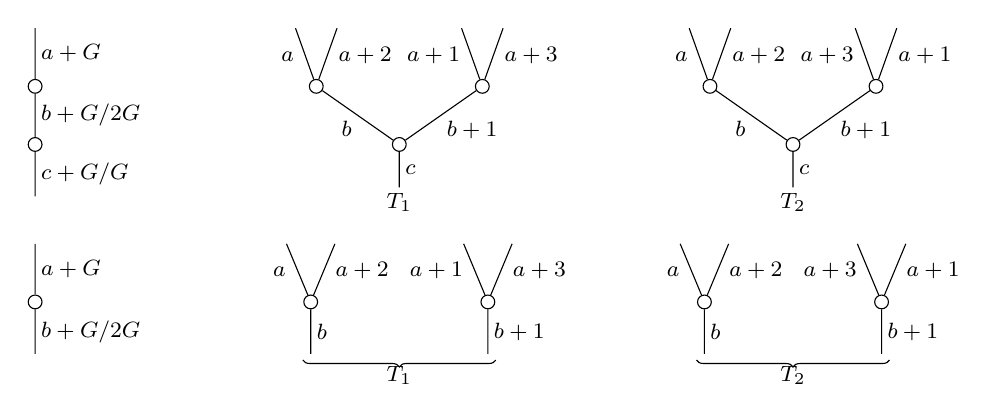
\begin{tikzpicture}[grow=up,auto,level distance=2.1em,
	every node/.style = {font=\footnotesize,inner sep=2pt},
	dummy/.style={circle,draw,inner sep=0pt,minimum size=1.75mm}]
		\node at (-1,0) {}
			child{node [dummy] {}
				child{node [dummy] {}
					child{
					edge from parent node [swap] {$a+G$}}
				edge from parent node [swap] {$b+G/2G$}}
			edge from parent node [swap] {$c + G/G$}};

		\node at  (3.625,0) {$T_1$}
			child{node [dummy] {}
				child[sibling distance = 6em]{node [dummy] {}
					child[sibling distance = 1.5em]{
					edge from parent node [swap,near end] {$a+3$}}
					child[sibling distance = 1.5em]{
					edge from parent node [near end] {$a+1$}}
				edge from parent node [swap] {$b+1$}}
				child[sibling distance = 6em]{node [dummy] {}
					child[sibling distance = 1.5em]{
					edge from parent node [swap,near end] {$a+2$}}
					child[sibling distance = 1.5em]{
					edge from parent node [near end] {$\phantom{0+}a$}}
				edge from parent node {$\phantom{1+}b$}}
			edge from parent node [swap] {$c$}};
		\node at  (8.625,0) {$T_2$}
			child{node [dummy] {}
				child[sibling distance = 6em]{node [dummy] {}
					child[sibling distance = 1.5em]{
					edge from parent node [swap,near end] {$a+1$}}
					child[sibling distance = 1.5em]{
					edge from parent node [near end] {$a+3$}}
				edge from parent node [swap] {$b+1$}}
				child[sibling distance = 6em]{node [dummy] {}
					child[sibling distance = 1.5em]{
					edge from parent node [swap,near end] {$a+2$}}
					child[sibling distance = 1.5em]{
					edge from parent node [near end] {$\phantom{0+}a$}}
				edge from parent node {$\phantom{1+}b$}}
			edge from parent node [swap] {$c$}};
		\node at (-1,-2) {}
			child{node [dummy] {}
				child[sibling distance=1.75em]{
				edge from parent node [swap]  {$a+G$}}
			edge from parent node [swap] {$b+G/2G$}};
		\node at (2.5,-2) {}
			child{node [dummy] {}
				child[sibling distance=1.75em]{
				edge from parent node [swap,near end] {$a+2$}}
				child[sibling distance=1.75em]{
				edge from parent node [near end]  {$\phantom{1+}a$}}
			edge from parent node [swap] {$b$}};
		\node at (4.75,-2) {}
			child{node [dummy] {}
				child[sibling distance=1.75em]{
				edge from parent node [swap,near end] {$a+3$}}
				child[sibling distance=1.75em]{
				edge from parent node [near end]  {$a+1$}}
			edge from parent node [swap] {$b+1$}};
		\draw[decorate,decoration={brace,amplitude=2.5pt}] (4.85,-2) -- (2.4,-2) node[midway]{$T_1$};
		\node at (7.5,-2) {}
			child{node [dummy] {}
				child[sibling distance=1.75em]{
				edge from parent node [swap,near end] {$a+2$}}
				child[sibling distance=1.75em]{
				edge from parent node [near end]  {$\phantom{1+}a$}}
			edge from parent node [swap] {$b$}};
		\node at (9.75,-2) {}
			child{node [dummy] {}
				child[sibling distance=1.75em]{
				edge from parent node [swap,near end] {$a+1$}}
				child[sibling distance=1.75em]{
				edge from parent node [near end]  {$a+3$}}
			edge from parent node [swap] {$b+1$}};
		\draw[decorate,decoration={brace,amplitude=2.5pt}] (9.85,-2) -- (7.4,-2) node[midway]{$T_2$};
	\end{tikzpicture}
\]

\end{example}




\subsection{Outer faces and tall maps}\label{OUTTALL SEC}

\subsection{Substitution}\label{SUBS SEC}

\bibliography{biblio}{}



\bibliographystyle{abbrv}



\end{document}